\section{Проектирование архитектуры системы}

\subsection{Общая архитектура системы}

\subsubsection{Роли узлов}

На верхнем уровне архитектуры выделяются два класса узлов: \emph{узлы
консенсуса (Raft-узлы)} и \emph{вычислительные узлы (workers)}. Такое
разделение соответствует распространённой практике отделения \emph{control
plane} (координация, согласование состояния, диспетчеризация) от
\emph{data/compute plane} (непосредственное выполнение пользовательских задач)
\cite{coulouris2012}.

Raft-узлы формируют кластер, поддерживающий реплицированную машину состояний,
принимают клиентские запросы, выполняют проверку/валидацию, принимают решения о
постановке задач в очередь и о распределении задач по воркерам, а также
обеспечивают линейризуемую (или близкую к ней) семантику наблюдения состояния.

Воркеры, в свою очередь, реализуют только «полезную работу»: исполняют выданные
задания в соответствии с политикой планировщика, периодически отчитываются о
прогрессе и возвращают результаты.

Архитектура приложения приложения приведена на рис.~\ref{fig:arch-overview}.

\begin{figure}
  \centering
  \includegraphics[scale=0.4]{inc/arch-overview.png}
  \caption{Высокоуровневая архитектура приложения}
  \label{fig:arch-overview}
\end{figure}

Данный подход минимизирует связанность компонентов: все операции записи в
«истину состояния» проходят через кластер Raft, а вычислительный контур
остаётся тонким и легко масштабируемым.

Это упрощает развитие системы (изменения протокола, эволюцию форматов,
миграции), повышает управляемость и упрощает доказательство корректности, так
как инварианты безопасности сосредоточены в одном месте — в реплицированной
машине состояний.

\subsubsection{Потоки управления и данные}

Клиент взаимодействует только с кластером Raft (запросы могут быть приняты
любым узлом и переадресованы лидеру). Каждая операция, которая влияет на
состояние системы (создание/отмена задания, изменение приоритета, отметка
результата), сначала записывается в лог кластера, подтверждается кворумом узлов
и \emph{только затем} применяется к машине состояний.

Из машины состояний изменения транслируются в модуль диспетчеризации (Task
manager), который назначает задания конкретным воркерам.

Обратный поток (результаты) также фиксируется через Raft перед тем, как станет
видимым для клиента.

Такая схема обеспечивает:
\begin{itemize}
    \item детерминированный порядок событий;
    \item устойчивость к повторам и сетевым артефактам за счёт идемпотентных
    идентификаторов задач;
    \item возможность повторного назначения задач при сбоях воркеров без
    нарушения согласованности.
\end{itemize}

\subsubsection{Обоснование отсутствия прямых связей между клиентом и рабочим узлом}

Исключение прямого клиентского трафика на воркеры и запрет горизонтальных
коммуникаций между воркерами снижает сложность системы и радиус отказа:

\begin{itemize}
  \item \textbf{Границы доверия и безопасность.} Все проверки
  аутентификации/авторизации, квоты, контроль нагрузки и согласование политик
  происходят в одном месте (в кластере Raft), что уменьшает поверхность атаки и
  упрощает аудит.
  \item \textbf{Единая точка сериализации.} Централизация записи в лог
  предотвращает расхождение состояний при разделениях сети и сбоях; воркеры не
  принимают решений, влияющих на глобальную консистентность.
  \item \textbf{Простота воркеров.} Воркеры могут оставаться без состояния
  (stateless) или слабосвязными по состоянию; замена/масштабирование происходит
  без координации между ними, что упрощает эксплуатацию.
  \item \textbf{Управляемое масштабирование.} Планирование, балансировка
  сосредоточены в кластере Raft; добавление воркеров линейно увеличивает
  пропускную способность без изменения протоколов согласования.
\end{itemize}

\subsubsection{Отказоустойчивость и модель сбоев}

Система проектируется под модель сбоев crash-stop/crash-recovery и частичной
синхронности сети.

Кластер Raft обеспечивает безопасность (отсутствие противоречивых коммитов) при
любой динамике и живучесть при выполнении допущений о времени
\cite{ongario2014}. Отказ отдельного воркера не влияет на целостность:
незавершённые задания остаются зафиксированными в состоянии и могут быть
переназначены. При отказе лидера выполняется переизбрание; после выбора нового
лидера система продолжает обслуживание запросов, как только будет достигнут
кворум. Такая конфигурация позволяет сохранять работоспособность при
недоступности до $\lfloor (N-1)/2 \rfloor$ узлов кластера консенсуса (для $N$ —
числа Raft-узлов), что является стандартной кворумной гарантией
\cite{lynch1996}.


\subsubsection{Масштабирование и управление нагрузкой}

Архитектура поддерживает независимое масштабирование плоскостей:
\begin{itemize}
  \item \textbf{Горизонтальный рост вычислительных мощностей.} Добавление воркеров
  увеличивает суммарные вычислительные мощности без влияния на алгоритм
  консенсуса.
  \item \textbf{Стабильность.} Количество Raft-узлов остаётся небольшим (обычно
  3–5) для минимизации латентности кворума и времени выборов
  \cite{ongario2014}.
\end{itemize}

\subsubsection{Рассмотренные альтернативы}

Были рассмотрены альтернативные топологии:

\begin{itemize}
\item прямое взаимодействие клиента с воркерами;
\item полно-связанная p2p-сетка воркеров с децентрализованным согласованием;
\item объединение ролей (каждый воркер — участник консенсуса).
\end{itemize}

От первого варианта отказались из-за роста поверхности ошибок и сложности
обеспечения глобальной согласованности. Второй вариант усложняет доказательство
корректности и эксплуатацию (динамика членства, маршрутизация, «горячие»
ключи). Третий ухудшает масштабирование: увеличение количества участников
консенсуса повышает латентность кворума и время выбора лидера.

Предложенная архитектура сохраняет консенсус компактным и управляемым, а
вычисления — эластичными и дешёвыми в масштабировании.

\subsection{Архитектура Raft узлов}

Каждый узел кластера Raft содержит несколько функциональных модулей,
взаимодействие которых обеспечивает корректную обработку запросов и поддержание
согласованного состояния всей системы. Архитектура узла изображена на
рис.~\ref{fig:arch-overview}.

\begin{figure}
  \centering
  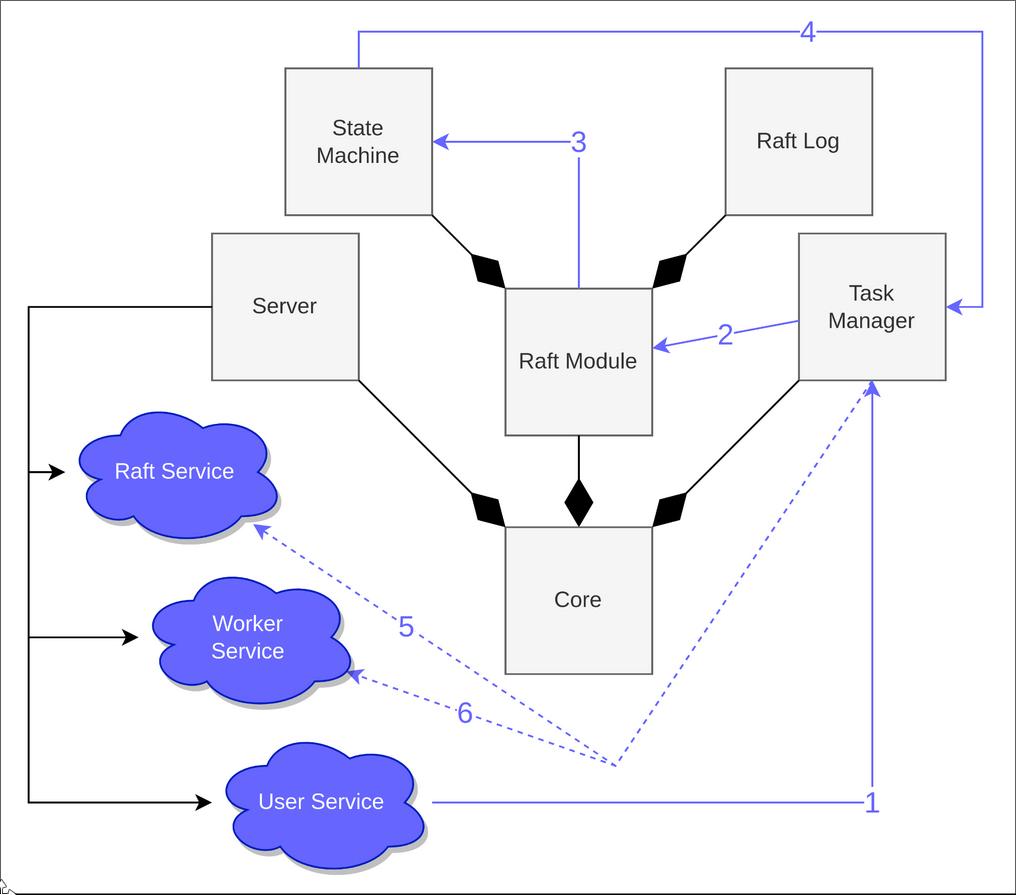
\includegraphics[scale=0.35]{inc/raft-arch.png}
  \caption{Архитектура Raft узла}
  \label{fig:arch-overview}
\end{figure}

Поток обработки клиентского запроса начинается с поступления данных на
\textbf{серверный модуль} узла-лидера. Сервер принимает запросы от клиентов и
маршрутизирует их во внутренние сервисы. В частности, запросы, связанные с
постановкой новых заданий на выполнение, направляются в
\textbf{пользовательский сервис (User Service)}, зарегистрированный в сервере.
Этот сервис выполняет первичную валидацию и подготовку данных, после чего
передаёт их в \textbf{менеджер заданий (Task Manager)}. Задача менеджера —
выбрать подходящий рабочий узел (worker) для выполнения поступившей задачи,
исходя из состояния системы, доступности ресурсов и стратегий планирования.

Поскольку система должна сохранять корректность работы даже при сбоях
отдельных узлов, Task Manager не отправляет задание воркеру напрямую.
Вместо этого сформированная операция передаётся в
\textbf{модуль Raft}, который отвечает за репликацию и согласование
состояния между всеми узлами кластера. Raft-модуль добавляет операцию
в \textbf{журнал Raft (Raft Log)}, который хранит все ещё не
зафиксированные изменения состояния. В рамках механизма Raft эти записи
реплицируются на все узлы кластера при очередных heartbeat-сообщениях
лидера.

Когда большинство (кворум) узлов подтверждает успешную запись данных в свои
локальные логи, лидер выполняет \textbf{коммит (commit)} — операцию переноса
записи в \textbf{машину состояний (State Machine)}. Машина состояний
представляет собой детерминированный автомат, который преобразует
последовательность закоммиченных операций в текущее состояние системы. За счёт
применения одной и той же последовательности команд на каждом узле достигается
консенсус — все реплики приходят к одинаковому результату независимо от того,
какой узел является лидером.

После того как операция фиксируется в машине состояний лидера, Task Manager
получает сигнал о возможности безопасного выполнения задания. На этом этапе
задание отправляется выбранному воркеру. Результат выполнения также проходит
через Raft: при завершении работы воркер формирует ответ, который реплицируется
и коммитится аналогично исходному запросу. Лишь после этого результат считается
подтверждённым и возвращается клиенту, что гарантирует согласованность даже при
отказах в момент ответа.

Ключевым элементом узла является \textbf{ядро (Core)}, которое выполняет роль
интеграционного слоя между модулями. Core отвечает за инициализацию и
завершение работы компонентов, координирует обмен сообщениями между ними и
предоставляет единый интерфейс для внешнего управления узлом.

Такая архитектура обеспечивает согласованное и детерминированное поведение
системы при сбоях, гарантирует, что любая операция либо применена на
большинстве узлов, либо будет проигнорирована. Система остаётся работоспособной
до тех пор, пока доступно более половины узлов кластера, что является базовым
требованием алгоритмов кворумного консенсуса.

\subsection{Архитектура клиентской части}

Клиентская часть системы обеспечивает пользователю удобный интерфейс
для постановки задач на выполнение и получения результатов.
Основными компонентами клиентской стороны являются:
\begin{itemize}
    \item \textbf{Конфигурационные данные задачи} — входные параметры,
    описывающие вычислительную задачу, хранятся в формате JSON
    (например, \texttt{data.json}). Такой формат выбран благодаря
    читаемости, простоте валидации и широкому распространению
    в экосистемах различных языков.
    \item \textbf{Библиотека задачи} — бинарный модуль
    (\texttt{libtask.so}), содержащий реализацию функции обработки данных.
    Такой подход позволяет передавать не только статические входные данные,
    но и сам алгоритм, который должен быть исполнен на воркере.
    \item \textbf{Клиентское приложение (CLI)} — консольная утилита,
    служащая интерфейсом между пользователем и распределённой системой.
    CLI принимает указанные входные файлы, сериализует их в формат,
    подходящий для сетевой передачи, и формирует запрос к кластеру Raft.
\end{itemize}

Процесс взаимодействия клиента с системой проходит следующие этапы (см.
рис.~\ref{fig:client-arch}):
\begin{enumerate}
    \item Пользователь передаёт клиенту \texttt{data.json} и
    динамическую библиотеку \texttt{libtask.so}, после чего CLI
    формирует запрос, содержащий данные задачи и код её исполнения,
    и отправляет его в кластер Raft.
    \item Лидер кластера принимает запрос, реплицирует его
    и передаёт в подсистему диспетчеризации, которая назначает
    задачу конкретному рабочему узлу. В запросе указывается
    уникальный идентификатор задачи для обеспечения идемпотентности.
    \item Клиент воркера получает задание и передаёт его на выполнение
    в среду исполнения, где подгружается \texttt{libtask.so} и
    запускается соответствующая функция с параметрами из \texttt{data.json}.
    После завершения выполнения результат формируется в сериализованном
    виде и отправляется обратно в кластер Raft для фиксации в состоянии.
    \item После коммита результата в реплицированной машине состояний
    лидер Raft уведомляет клиента о завершении работы. CLI принимает
    ответ, сохраняет результат локально либо выводит пользователю
    в удобной форме.
\end{enumerate}

\begin{figure}
  \centering
  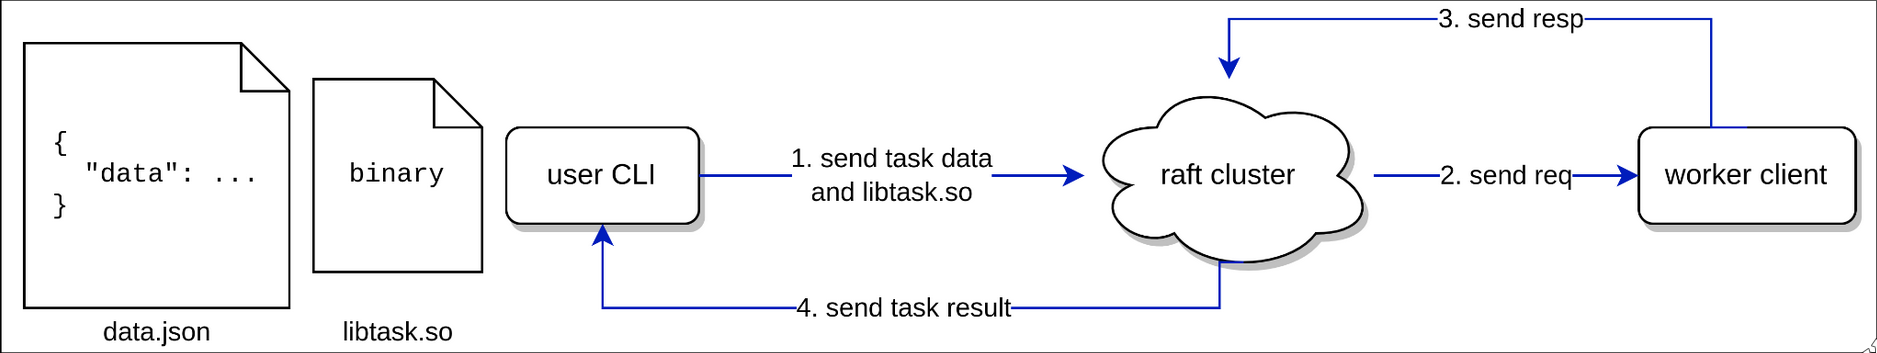
\includegraphics[scale=0.25]{inc/client-arch.png}
  \caption{Взаимодействие клиента с кластером}
  \label{fig:client-arch}
\end{figure}

Данная архитектура клиентской части обладает рядом преимуществ:
\begin{itemize}
    \item \textbf{Универсальность.} Клиент не привязан к конкретному
    типу задач — любое вычисление, представленное в виде бинарной
    библиотеки с единым интерфейсом, может быть передано в систему.
    \item \textbf{Минимальные зависимости.} Клиент реализован как
    лёгкая утилита, не требующая сложной конфигурации;
    это упрощает её развёртывание и интеграцию в CI/CD.
    \item \textbf{Надёжность.} Все этапы (от постановки задачи до
    получения ответа) проходят через механизм Raft, что гарантирует
    сохранность данных даже при сбоях сети или падении узлов.
\end{itemize}

Таким образом, клиентская часть системы выступает удобным
и унифицированным интерфейсом, который инкапсулирует сложность
взаимодействия с распределённой инфраструктурой и позволяет
пользователю сосредоточиться на определении вычислительных задач
и анализе результатов.

\subsection{Архитектура вычислительного узла}

Вычислительный узел предназначен для непосредственного выполнения задач,
поступающих из кластера Raft, и возврата результатов их обработки. Архитектура
воркера организована таким образом, чтобы обеспечить изоляцию вычислений,
устойчивость к сбоям и минимальное влияние выполняемой задачи на стабильность
основной службы.

Ключевые компоненты вычислительного узла:
\begin{itemize}
    \item \textbf{Главный процесс (main)} — точка входа, отвечающая за
    инициализацию среды, запуск клиента воркера и менеджера процессов. Главный
    процесс контролирует жизненный цикл остальных компонентов и обеспечивает их
    перезапуск при сбоях.
    \item \textbf{Клиент воркера (worker client)} — процесс, который
    поддерживает постоянное соединение с кластером Raft, принимает задания на
    выполнение и уведомляет менеджер о необходимости запуска вычислительных
    контейнеров.
    \item \textbf{Менеджер (manager)} — отдельный процесс, отвечающий за
    создание изолированных рабочих процессов (\textbf{mayfly}), которым
    передаётся выполнение конкретных задач. Такой подход снижает риск
    повреждения памяти или зависания основного сервиса из-за некорректного кода
    задачи.
    \item \textbf{Mayfly-процесс} — лёгкий дочерний процесс, который выполняет
    задачу. На этапе инициализации загружает указанную динамическую библиотеку,
    выполняет функцию обработки данных и формирует результат.
\end{itemize}

Поток выполнения задачи организован следующим образом (см.
рис~\ref{fig:worker-arch}):

\begin{enumerate}
    \item \textbf{Приём запроса.} Worker client получает задание
    из кластера Raft и подтверждает его приём.
    \item \textbf{Создание рабочего процесса.} Worker client
    отправляет запрос менеджеру на создание нового mayfly-процесса.
    Менеджер выполняет \texttt{fork()}, создавая изолированный процесс.
    \item \textbf{Загрузка библиотеки.} Mayfly-процесс подгружает
    указанную пользователем библиотеку задачи (по имени, переданному
    в запросе).
    \item \textbf{Выполнение задачи.} Обработка входных данных
    производится внутри mayfly-процесса.
    В случае ошибки или аварийного завершения процесс завершается
    без влияния на основной клиент воркера.
    \item \textbf{Отправка результата.} После завершения выполнения
    результат возвращается менеджеру, который передаёт его обратно
    в worker client.
    \item \textbf{Репликация результата.} Worker client формирует
    ответ и отправляет его в кластер Raft для фиксации в
    реплицированной машине состояний.
\end{enumerate}

\begin{figure}
  \centering
  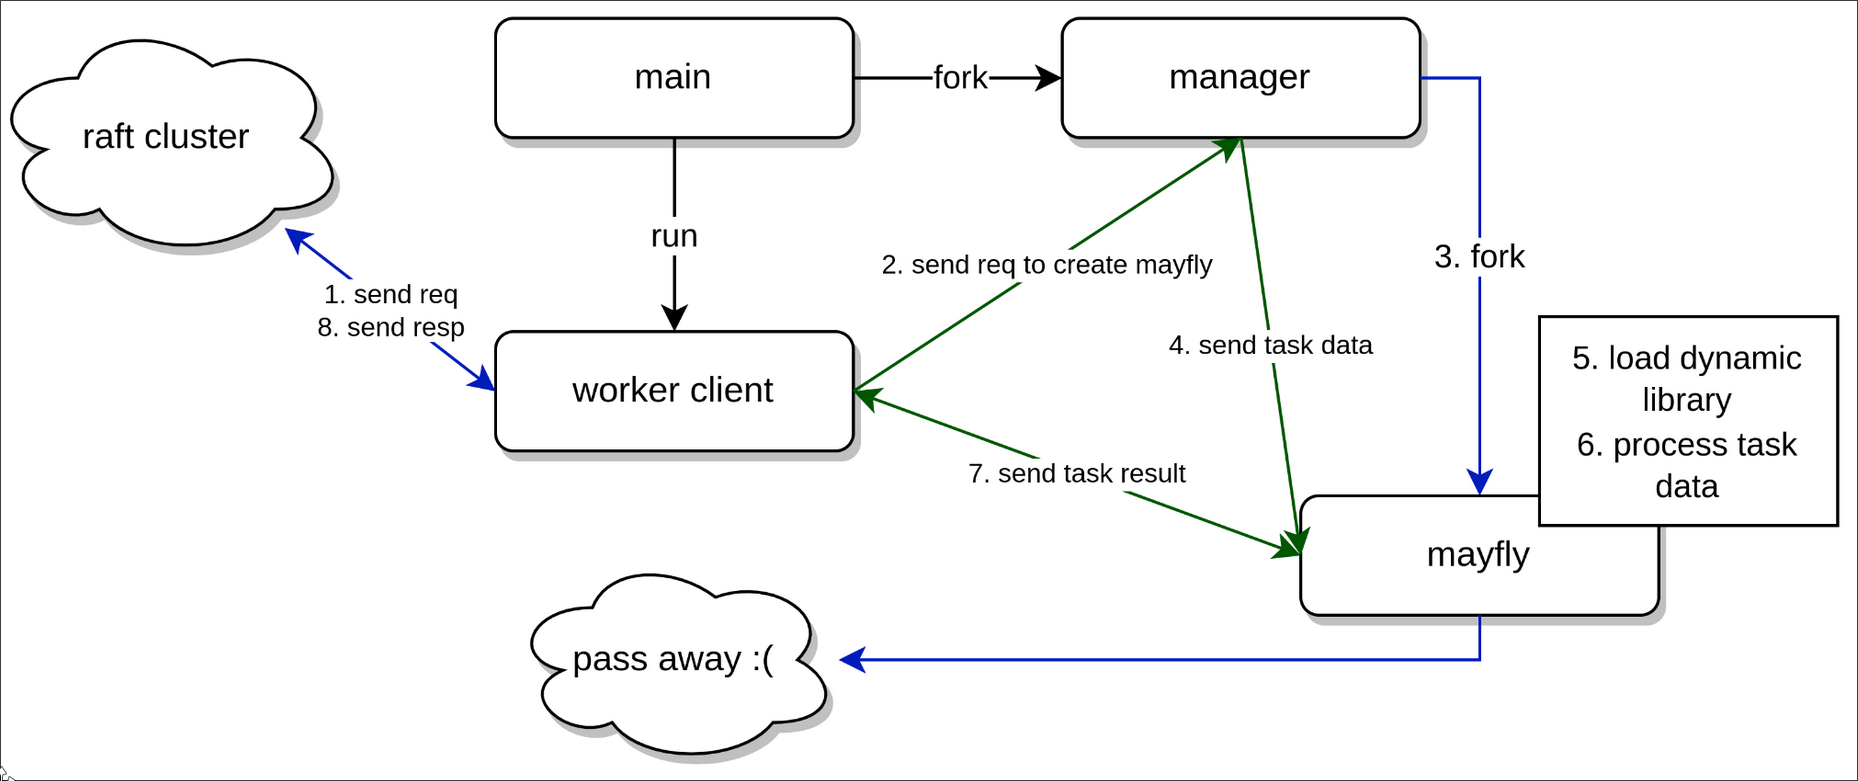
\includegraphics[scale=0.25]{inc/worker-arch.png}
  \caption{Взаимодействие вычислительного узла с кластером}
  \label{fig:worker-arch}
\end{figure}

Архитектура поддерживает модель «одно задание — один процесс», что
обеспечивает:

\begin{itemize}
    \item \textbf{Изоляцию исполнения}: сбой в задаче не влияет
    на остальные процессы воркера;
    \item \textbf{Высокую отказоустойчивость}: при завершении
    дочернего процесса менеджер может корректно обработать сбой,
    зарегистрировать ошибку и при необходимости запросить
    повторное выполнение через кластер;
    \item \textbf{Простоту очистки ресурсов}: после завершения работы
    mayfly-процесс уничтожается вместе с выделенными ресурсами,
    исключая утечки памяти.
\end{itemize}

Такое построение вычислительного узла обеспечивает гибкость и устойчивость всей
системы, позволяя безопасно выполнять пользовательский код, динамически
масштабировать количество обрабатываемых задач и гарантировать возврат
результата даже при частичных сбоях.
